\section{TF package} \label{sec:tf_package}
The TF package is used to keep track of coordinate frames over time in a tree structure. It transforms points or vectors between two frames at any particular point in time. The Turtlebot has coordinate frames setup for the "base\_link" and its different sensors. The implemented design of the Turtlebot has a RealSense camera facing backward and two Sick LIDARs on the sides. The design can be seen in figure \ref{fig:robot_tf}.

\begin{figure}[H]
    \centering
    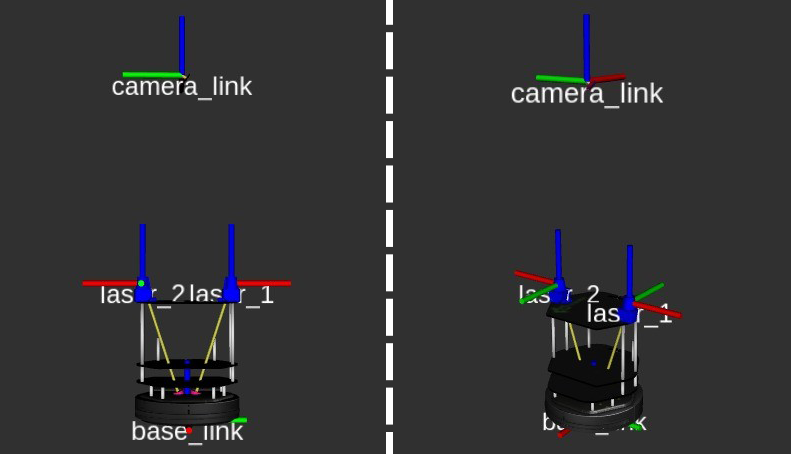
\includegraphics[width=\textwidth]{figures/robotTF.png}
    \caption{Figures are showing the base\_link, laser\_1, laser\_2 and camera\_link frames on the model of the Turtlebot from the front. Left figure is from the front. Right figure is from the side.}
    \label{fig:robot_tf}
\end{figure}

The camera and LIDAR frames have to be defined and established in TF to build a relationship between the different coordinate frames of the system. TF defines transformations between "parent" frame and "child" frame. Here, the parent frame is setup to be the "base\_link" of the Turtlebot, which is defined to be around the axis of rotation of the wheels. The child frame is the "laser" frame for the lidar and the "camera" frame for the camera. Since there are two LIDARs, the frames were called "laser\_1" and "laser\_2". The two LIDARs are parallel to each other and oriented away from each other on the Turtlebot. The frames are defined in $x$, $y$, $z$ and roll, pitch, yaw according to the right hand rule and the units are in SI units.


\begin{table}[H]
\centering
\begin{tabular}{@{}l|c|c|c|c|c|c|@{}}
\cline{2-5}
& \cellcolor[HTML]{DBDBDB}X & \cellcolor[HTML]{DBDBDB}Y & \cellcolor[HTML]{DBDBDB}Z & \cellcolor[HTML]{DBDBDB}Roll & \cellcolor[HTML]{DBDBDB}Pitch & \cellcolor[HTML]{DBDBDB}Yaw \\ \hline
\multicolumn{1}{|l|}{\cellcolor[HTML]{DBDBDB}Laser\_1} & 0.00 & 0.15 & 0.46 & 0.00 & 0.00 & $\pi$/2\\ \hline
\multicolumn{1}{|l|}{\cellcolor[HTML]{DBDBDB}Laser\_2} & 0.00 & -0.15 & 0.46 & 0.00 & 0.00 & $-\pi$/2\\ \hline
\multicolumn{1}{|l|}{\cellcolor[HTML]{DBDBDB}Camera\_link} & 0.00 & 0.00 & 1.30 & 0.00 & 0.00 & $\pi$\\ \hline
\end{tabular}
\caption{Table of coordinates relative to the base\_link, (x, y, z) represented in meters and (roll, pitch, yaw) in radians.}
\label{fig:coordiantetable}
\end{table}


The LIDAR laser frames are located 0.46 meters on the $z$-axis of the "base\_link" frame, oriented $\pm \pi/2$. Whereas the camera frame is 1.30 meters away on the z from the "base\_link" frame, oriented $\pm \pi$.

In the "turtlebot\_description" package, a new robot description were a added. This was done by first including macros that describe the different parts of the robot such as the Kobuki base, the hexagon plates that form the Turtlebot, the Intel Real Sense D435 camera as well as the SICK LIDARs. Afterwards, the different macros are defined by specifying, if needed, a list of parameters that were declared in the macro description of the part. Some of the parameters are the parent frame, x, y, or z offset in addition to roll, pitch and yaw for specifying the orientation between the frames of the parts in order to connect them in a TF tree structure.